%%%%%%%%%%%%%%%%%%%%%%%
%% Folie             %%
%%%%%%%%%%%%%%%%%%%%%%%
\begin{frame}
    \frametitle{Goals Guided Research}

\begin{PraesentationAufzaehlung}
    \item Implementation of I2A
    \item 
\end{PraesentationAufzaehlung}

\end{frame}
\clearpage

%%%%%%%%%%%%%%%%%%%%%%%
%% Folie             %%
%%%%%%%%%%%%%%%%%%%%%%%
\begin{frame}
    \frametitle{Goals Guided Research}

\begin{PraesentationAufzaehlung}
    \item Implementation of I2A
    \item 
\end{PraesentationAufzaehlung}

\end{frame}
\clearpage



%%%%%%%%%%%%%%%%%%%%%%%
%% Folie             %%
%%%%%%%%%%%%%%%%%%%%%%%
\begin{frame}
    \PraesentationUeberschriftZweizeilig{Imagination-Augmented Agent (I2A)}{Weber et al.(2017)}

\begin{PraesentationAufzaehlung}
    \item Architecture for deep reinforcement learning
    \item Imaginate the future and do better action based on this
    \item Combine model-free and model-based aspects
\end{PraesentationAufzaehlung}

\end{frame}
\clearpage

%%%%%%%%%%%%%%%%%%%%%%%%%%%%%%%%%%%%%%%%
%% Folie: Bilder                      %%
%%%%%%%%%%%%%%%%%%%%%%%%%%%%%%%%%%%%%%%%
\begin{frame}
    \frametitle{I2A Architecture}


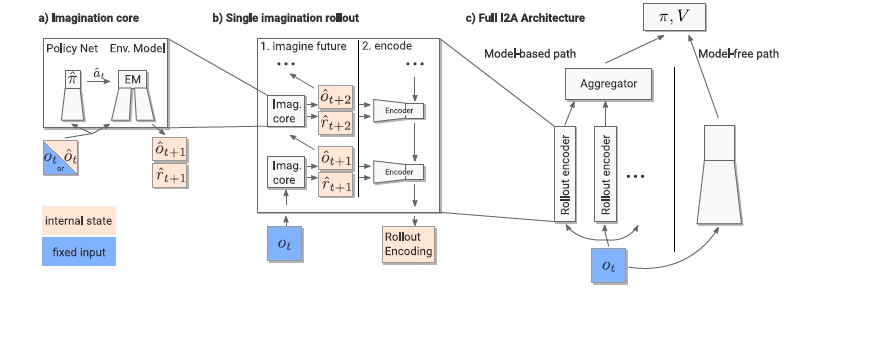
\includegraphics[width=\columnwidth]{./Images/i2a_architecture.png}%

    
\end{frame}
\clearpage

%%%%%%%%%%%%%%%%%%%%%%%%%%%%%%%%%%%%%%%%
%% Folie: Bilder                      %%
%%%%%%%%%%%%%%%%%%%%%%%%%%%%%%%%%%%%%%%%
\begin{frame}
    \frametitle{I2A Architecture - Model Free Path}


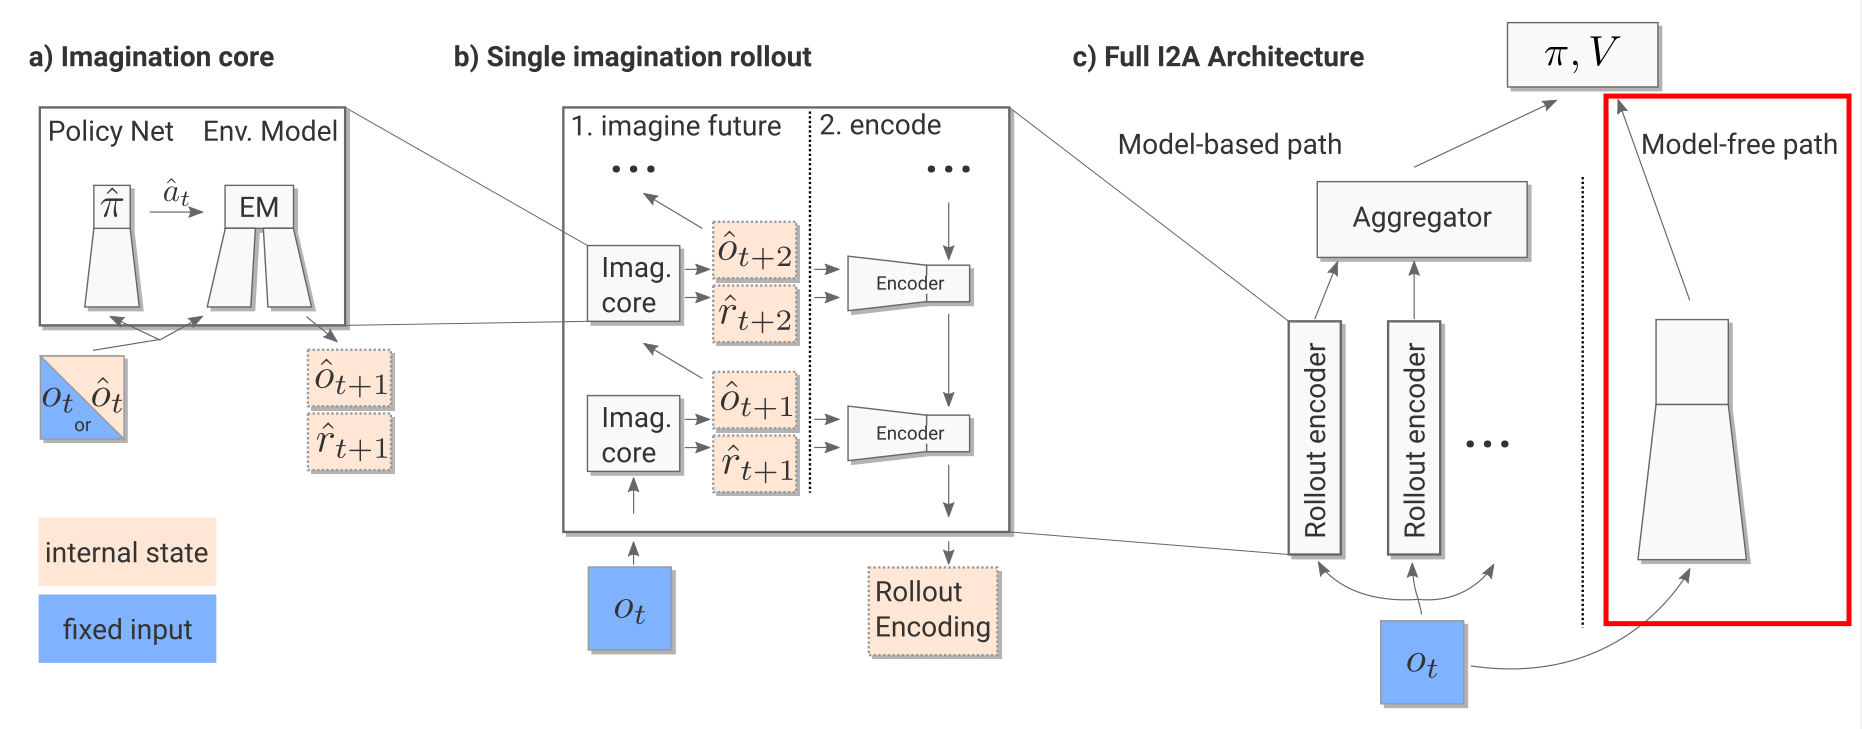
\includegraphics[width=\columnwidth]{./Images/i2a_all_model_free_path.png}%

\begin{PraesentationAufzaehlung}
	\item Advantage-Actor-Critic (A2C)
\end{PraesentationAufzaehlung}

\end{frame}
\clearpage

%%%%%%%%%%%%%%%%%%%%%%%%%%%%%%%%%%%%%%%%
%% Folie: Bilder - Zweispaltige Seite %%
%%%%%%%%%%%%%%%%%%%%%%%%%%%%%%%%%%%%%%%%
\begin{frame}
    \frametitle{I2A Architecture - Model Free Path}

\begin{multicols}{2}
	\begin{PraesentationAufzaehlung}
		\item Advantage-Actor-Critic (A2C)
	\end{PraesentationAufzaehlung}
    \vfill\columnbreak
	\begin{center}
    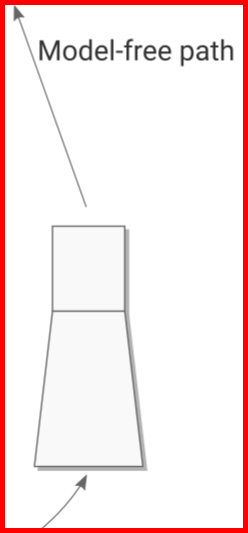
\includegraphics[height=.5\textheight]{./Images/i2a_model_free_path.png}%
	\end{center}
\end{multicols}
    
\end{frame}
\clearpage


%%%%%%%%%%%%%%%%%%%%%%%%%%%%%%%%%%%%%%%%
%% Folie: Bilder                      %%
%%%%%%%%%%%%%%%%%%%%%%%%%%%%%%%%%%%%%%%%
\begin{frame}
    \frametitle{I2A Architecture - Model Based Path}


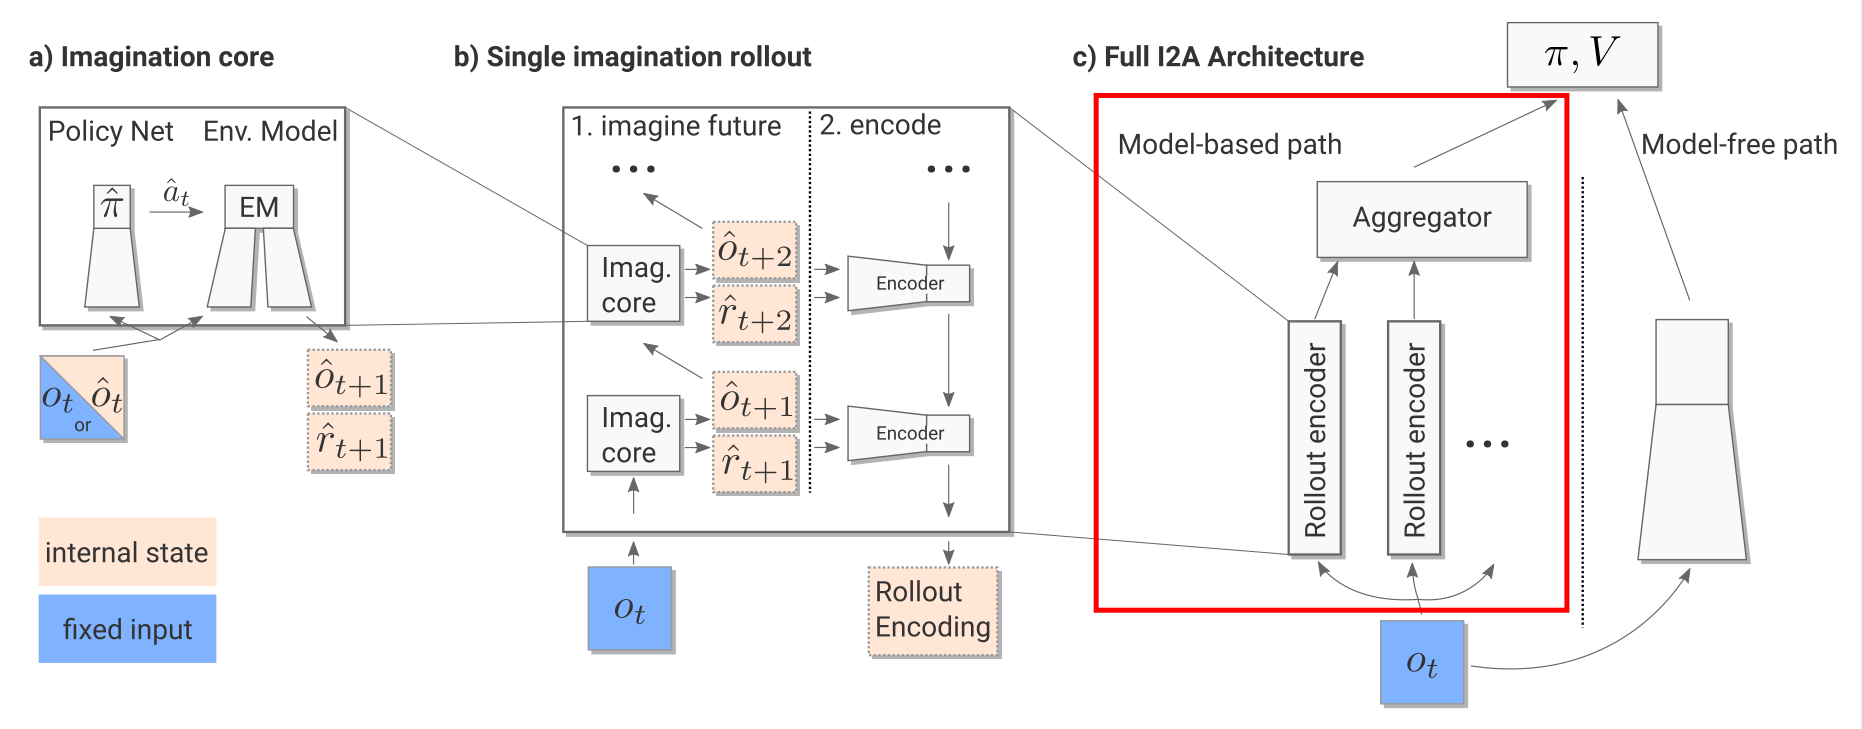
\includegraphics[width=\columnwidth]{./Images/i2a_all_model_based_path.png}%

\begin{PraesentationAufzaehlung}
	\item Imaginate the Future and use this information for desission making
\end{PraesentationAufzaehlung}
    
\end{frame}
\clearpage

%%%%%%%%%%%%%%%%%%%%%%%%%%%%%%%%%%%%%%%%
%% Folie: Bilder - Zweispaltige Seite %%
%%%%%%%%%%%%%%%%%%%%%%%%%%%%%%%%%%%%%%%%
\begin{frame}
    \frametitle{I2A Architecture - Model Based Path}

\begin{multicols}{2}
	\begin{PraesentationAufzaehlung}
	    \item Rollout encoder:\\
		Imaginate the Future and learn relevent information that can happen
		\item Aggregator: \\
		Concatitate the rollouts
	\end{PraesentationAufzaehlung}
    \vfill\columnbreak
	\begin{center}
    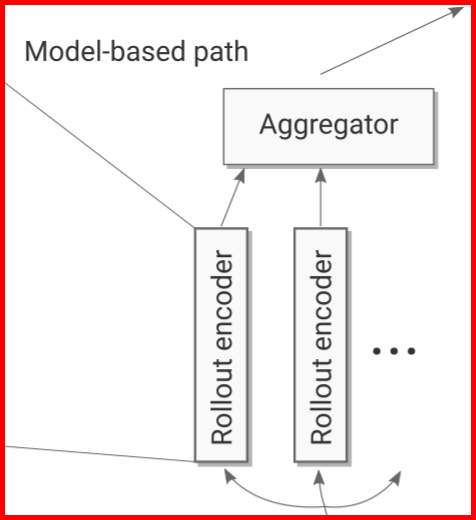
\includegraphics[height=.5\textheight]{./Images/i2a_model_based.png}%
	\end{center}
\end{multicols}
    
\end{frame}
\clearpage


%%%%%%%%%%%%%%%%%%%%%%%%%%%%%%%%%%%%%%%%
%% Folie: Bilder                      %%
%%%%%%%%%%%%%%%%%%%%%%%%%%%%%%%%%%%%%%%%
\begin{frame}
    \frametitle{I2A Architecture - Imagination Rollout}


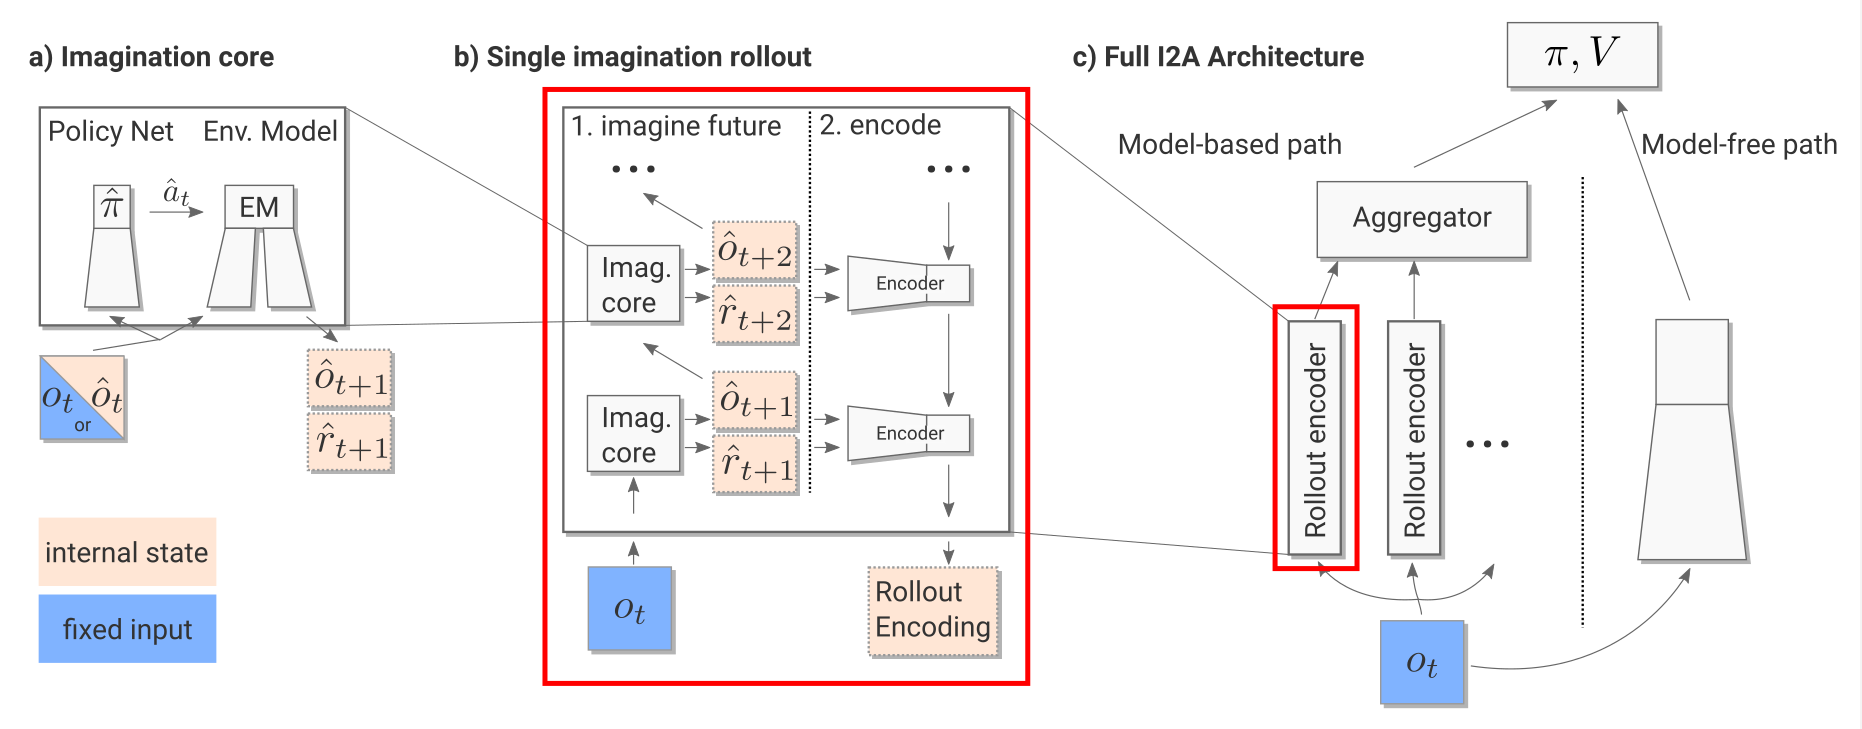
\includegraphics[width=\columnwidth]{./Images/i2a_all_imagination_rollout.png}%

\begin{PraesentationAufzaehlung}
	\item Predict what will happen in the future
\end{PraesentationAufzaehlung}
    
\end{frame}
\clearpage


%%%%%%%%%%%%%%%%%%%%%%%%%%%%%%%%%%%%%%%%
%% Folie: Bilder - Zweispaltige Seite %%
%%%%%%%%%%%%%%%%%%%%%%%%%%%%%%%%%%%%%%%%
\begin{frame}
    \frametitle{I2A Architecture - Imagination Future}

\begin{multicols}{2}
	\begin{PraesentationAufzaehlung}
		\item Imagine Future:\\
		Rollout the future for an input observation
	    \item Imagination Core:\\
		Imaginate the next observation $o_{t+i}$ and the next reward $r_{t+i}$
	\end{PraesentationAufzaehlung}
    \vfill\columnbreak
	\begin{center}
    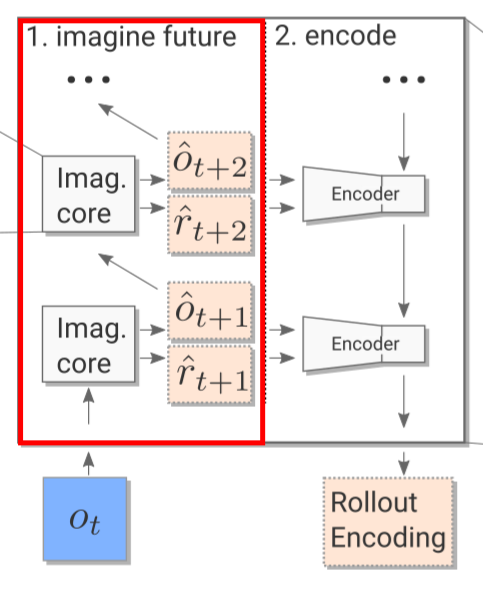
\includegraphics[height=.5\textheight]{./Images/imagine_future.png}%
	\end{center}
\end{multicols}
    
\end{frame}
\clearpage

%%%%%%%%%%%%%%%%%%%%%%%%%%%%%%%%%%%%%%%%
%% Folie: Bilder - Zweispaltige Seite %%
%%%%%%%%%%%%%%%%%%%%%%%%%%%%%%%%%%%%%%%%
\begin{frame}
    \frametitle{I2A Architecture - Encoder}

\begin{multicols}{2}
	\begin{PraesentationAufzaehlung}
		\item Encoder:\\
		CNN Network followed by an LSTM Network\\
		Learns usefull information from the rollouts
	\end{PraesentationAufzaehlung}
    \vfill\columnbreak
	\begin{center}
    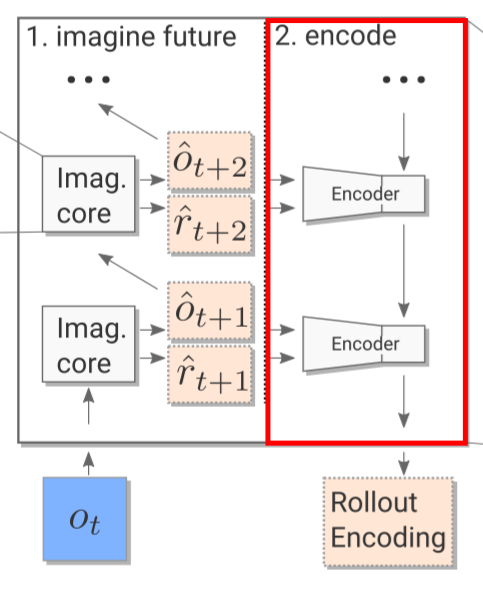
\includegraphics[height=.5\textheight]{./Images/encoder.png}%
	\end{center}
\end{multicols}
    
\end{frame}
\clearpage

%%%%%%%%%%%%%%%%%%%%%%%%%%%%%%%%%%%%%%%%
%% Folie: Bilder                      %%
%%%%%%%%%%%%%%%%%%%%%%%%%%%%%%%%%%%%%%%%
\begin{frame}
    \frametitle{I2A Architecture - Imagination Core}


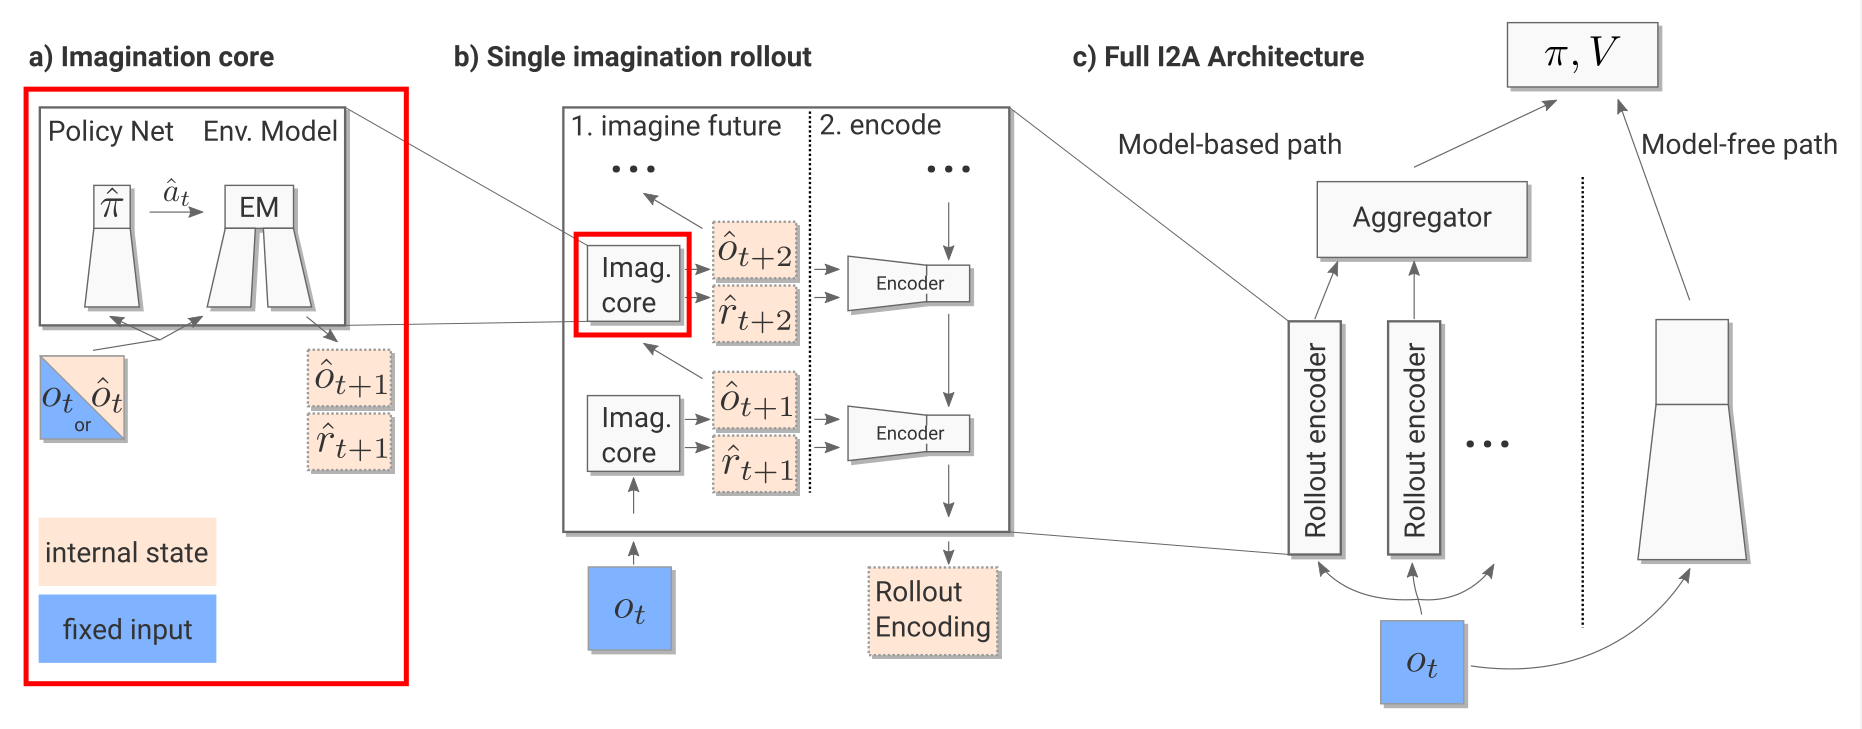
\includegraphics[width=\columnwidth]{./Images/i2a_all_imagination_core.png}%

    
\end{frame}
\clearpage


%%%%%%%%%%%%%%%%%%%%%%%%%%%%%%%%%%%%%%%%
%% Folie: Bilder - Zweispaltige Seite %%
%%%%%%%%%%%%%%%%%%%%%%%%%%%%%%%%%%%%%%%%
\begin{frame}
    \frametitle{I2A Architecture - Imagination Core}

\begin{multicols}{2}
	\begin{PraesentationAufzaehlung}
	    \item Imaginate the next observation $o_{t+i}$ and the next reward $r_{t+i}$
	\end{PraesentationAufzaehlung}
    \vfill\columnbreak
	\begin{center}
    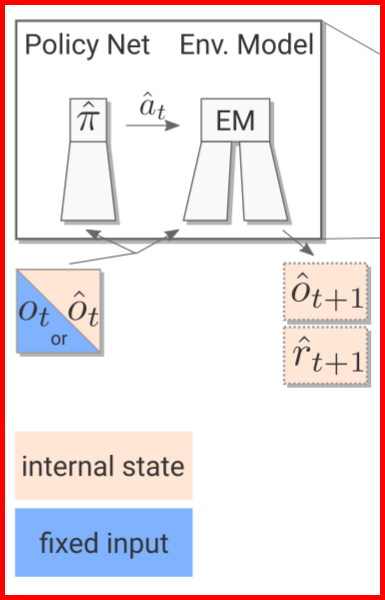
\includegraphics[height=0.5\textheight]{./Images/i2a_imagination_core.png}%
	\end{center}
\end{multicols}
    
\end{frame}
\clearpage

%%%%%%%%%%%%%%%%%%%%%%%%%%%%%%%%%%%%%%%%
%% Folie: Bilder - Zweispaltige Seite %%
%%%%%%%%%%%%%%%%%%%%%%%%%%%%%%%%%%%%%%%%
\begin{frame}
    \frametitle{I2A Architecture - Policy Network}

\begin{multicols}{2}
	\begin{PraesentationAufzaehlung}
	    \item policy network $\pi$
		desides the next action $a_t$
	\end{PraesentationAufzaehlung}
    \vfill\columnbreak
	\begin{center}
    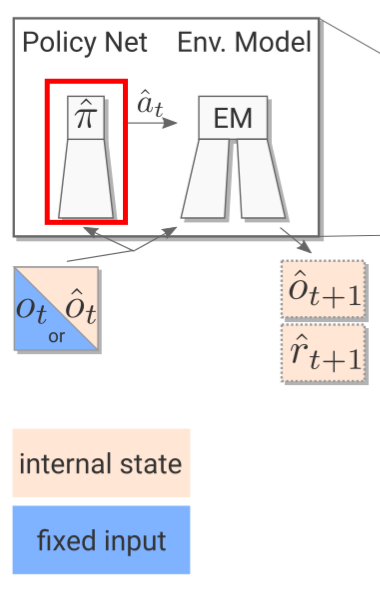
\includegraphics[height=0.5\textheight]{./Images/policy.png}%
	\end{center}
\end{multicols}
    
\end{frame}
\clearpage

%%%%%%%%%%%%%%%%%%%%%%%%%%%%%%%%%%%%%%%%
%% Folie: Bilder - Zweispaltige Seite %%
%%%%%%%%%%%%%%%%%%%%%%%%%%%%%%%%%%%%%%%%
\begin{frame}
    \frametitle{I2A Architecture - Environment Model}

\begin{multicols}{2}
	\begin{PraesentationAufzaehlung}
		\item environment model EM imaginate what will happen if we are in state $o_t$ and do action $a_t$
	\end{PraesentationAufzaehlung}
    \vfill\columnbreak
	\begin{center}
    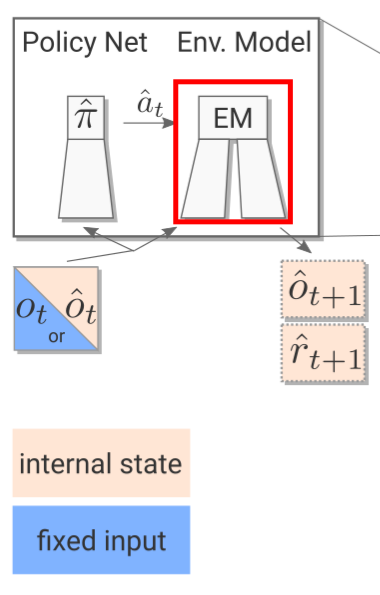
\includegraphics[height=0.5\textheight]{./Images/environment_model.png}%
	\end{center}
\end{multicols}
    
\end{frame}
\clearpage

%%%%%%%%%%%%%%%%%%%%%%%%%%%%%%%%%%%%%%%%
%% Folie: Bilder - Zweispaltige Seite %%
%%%%%%%%%%%%%%%%%%%%%%%%%%%%%%%%%%%%%%%%
\begin{frame}
    \frametitle{I2A Architecture - Environment Model Architecture}

\begin{multicols}{2}
	\begin{PraesentationAufzaehlung}
		\item kind of Autoencoder
		\item input:\\
		stack of last 3 observations\\
		action as one hot vector
	\end{PraesentationAufzaehlung}
    \vfill\columnbreak
	\begin{center}
    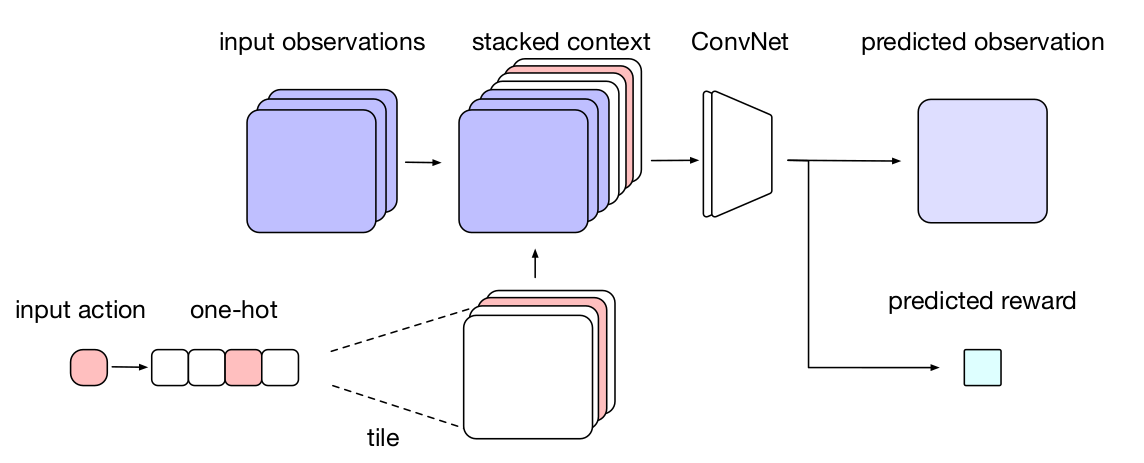
\includegraphics[width=\columnwidth]{./Images/environment_model_architecture.png}%
	\end{center}
\end{multicols}
    
\end{frame}
\clearpage


%%%%%%%%%%%%%%%%%%%%%%%%%%%%%%%%%%%%%%%%%%%%%%%%%%%%% 
 
 % FOLIENSTIL: Weisse Schrift auf blauem Grund 
\PraesentationMasterWeissBlau 
\begin{frame} 
    \frametitle{MiniPacman}
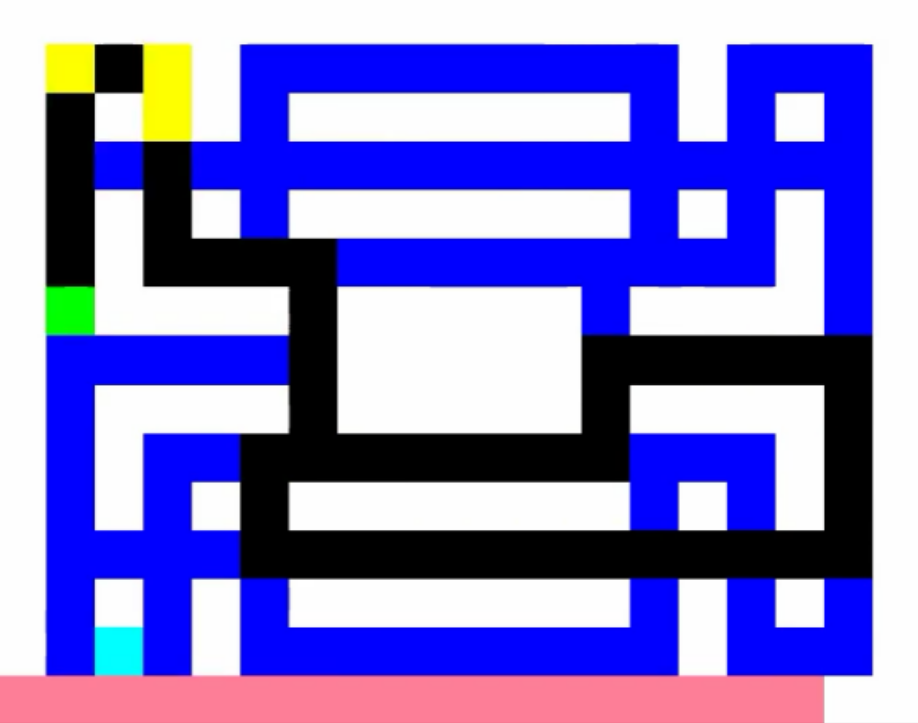
\includegraphics[height=0.5\textheight]{./Images/mini_pacman.png}%
\end{frame} 

\PraesentationMasterStandard

%%%%%%%%%%%%%%%%%%%%%%%%%%%%%%%%%%%%%%%%
%% Folie: Bilder - Zweispaltige Seite %%
%%%%%%%%%%%%%%%%%%%%%%%%%%%%%%%%%%%%%%%%
\begin{frame}
    \frametitle{MiniPacman}

\begin{PraesentationAufzaehlung}
	\item 15 * 19 Grid World
	\item different modes
\end{PraesentationAufzaehlung}
    
\end{frame}
\clearpage




